\documentclass[11pt]{book}
\usepackage[spanish]{babel}
\usepackage{comfortaa}
\usepackage[T1]{fontenc}
\renewcommand*\oldstylenums[1]{{\firaoldstyle #1}}
\usepackage[T1]{fontenc}
\usepackage[utf8]{inputenc}
\usepackage[letterpaper]{geometry} % Custom margins
\usepackage[colorlinks = true,linkcolor = blue]{hyperref}
\usepackage[dvipsnames,table]{xcolor} % Required for custom color
\usepackage{graphicx}
\usepackage{tabularx}
\usepackage{multicol,multirow}
\usepackage{float}
\usepackage{remreset}
\usepackage{enumitem}
\usepackage{xparse}
\usepackage{wrapfig}
\usepackage{amssymb,amsmath}
\usepackage{tikz}
\usepackage{subfiles}
\input{insbox}
\usepackage{etoolbox}
\setlength{\parindent}{0pt}
\graphicspath{{./Images}} %Setting the graphicspath
\definecolor{colorrds}{HTML}{0060A0} % Custom colour
\usetikzlibrary{
  arrows,
  positioning,
  matrix,
  calc,
  decorations.pathreplacing,
  decorations.pathmorphing,
  decorations.markings,
  decorations.text,
  shapes,
  backgrounds,
  shadows,
  trees,
  fit,
  snakes,
  patterns,
  mindmap,
  intersections,
  calendar,
  plotmarks,
  spy,
  tikzmark}

  \tikzset{
  abstractbox/.style={
    draw=black, fill=white, rectangle, 
    inner sep=12pt, style=rounded corners,
    drop shadow={fill=black, opacity=1}
  },
  abstracttitle/.style={fill=white}
}

  \decimalpoint
  \makeatletter
  \def\maxwidth{%
    \ifdim\Gin@nat@width>\linewidth
      \linewidth
    \else
      \Gin@nat@width
    \fi
  }
  \makeatother
%%%% APRENDISAJES TEXTBOX
\tikzset{
  abstractbox/.style={
    draw=black, fill=white, rectangle, 
    inner sep=12pt, style=rounded corners,
    drop shadow={fill=black, opacity=1}
  },
  abstracttitle/.style={fill=white}
}
\newcommand{\boxabstract}[2][fill=white]{
  \begin{tikzpicture}
    \node [abstractbox, #1] (box)
    {\begin{minipage}{0.9\linewidth}
        \setlength{\parindent}{2mm} % Indentar.
        \normalfont #2
      \end{minipage}};
    \node[abstracttitle, right=10pt] at (box.north west) {Aprendizajes esperados:};
    \node[draw=none, fit=(box)] {};
  \end{tikzpicture}
}%
%%%%%%%%%%%%%%%%%%%%%%%%

\makeatletter
  \@removefromreset{section}{chapter}
\makeatother
\addto\captionsspanish{\renewcommand{\chaptername}{}}
\renewcommand{\thechapter}{Unidad \arabic{chapter}}
\renewcommand{\thesection}{S\arabic{section}}
\renewcommand{\thesubsection}{L\arabic{subsection}}
\setlength{\parindent}{0pt}

%%%%%%%%%%%%% START questions env
%Idea from https://tex.stackexchange.com/a/236668/1952
\DeclareDocumentCommand\question{o}{%
    \item\IfNoValueTF{#1}{}{(#1 puntos)}}
\newenvironment{questions}[1][]{\enumerate[,#1]}{\endenumerate}
\newlist{oneparchoices}{enumerate*}{1}
\setlist[oneparchoices,1]{label=\quad\alph*), itemjoin={{\quad}}}
\newlist{choices}{enumerate*}{1}
\setlist[choices,1]{label=\quad$\square$, itemjoin={{\\}},leftmargin = 1cm}
\newcommand{\choice}{\item}
%%%%%%%%%%%%% END questions env
\newenvironment{mybox}[3][]{%
  \begin{tikzpicture}[#1]%
    \def\myboxname{#3}%
    % good options: minimum height, minimum width
    \node [draw, inner sep=2ex,  align=justify]
      (BOXCONTENT) \bgroup\rule{0ex}{0ex}\ignorespaces
  }{%
    \egroup;
    \node [right, inner sep=3pt, fill=colorrds!75, outer sep=0pt, 
      text height=2ex, text depth=.5ex] (BOXNAME) 
      at ([shift={(-1em,5pt)}]BOXCONTENT.north west) {\myboxname};
    \fill[colorrds] (BOXNAME.north east) -- +(-1em,1em)
      -- +(-1em,0) -- cycle;
    \fill[colorrds] (BOXNAME.south west) -- +(1em,-1em)
      -- +(1em,0) -- cycle;
  \end{tikzpicture}
}\begin{document}
\pagestyle{empty}
\newgeometry{left=15mm,top=50mm,bottom=0mm} % Custom margins
\begin{center}
  {\Huge F\'isica}\\
  \vspace{2cm}
  \normalsize
  \textbf{\large Cuaderno de trabajo}\\
  para los alumnos de 2$^\circ$ de  Secundaria\\
  en el curso durante el ciclo escolar\\
  \textbf{2022-2023}\\
  \vspace{2.5cm}
  \small POR\\
  \Large J. C. Melchor Pinto\\[0.5em]
  \normalsize Profesor de asignatura en\\
  \vspace{1cm}
  
\includegraphics[width=4cm]{./Unidad 2/Images/LOGO_RDS_nobg}
\end{center}
\vspace{2cm}
%\include*{Functional/TitlePage}
\hspace{-16mm}
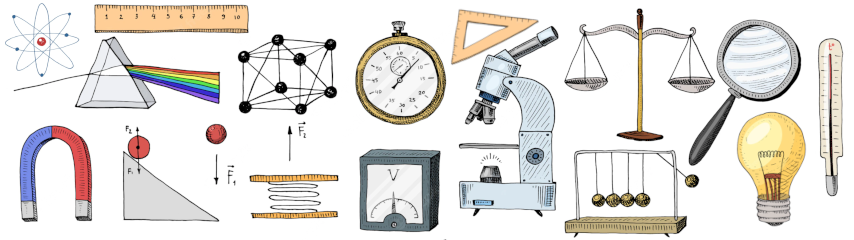
\includegraphics[width=\paperwidth]{./Unidad 2/Images/cover_bg}
\restoregeometry%
\tableofcontents
\chapter{}

\section{Tecnolog\'ia y transformaci\'on de la sociedad}
\subsection{El cambio y el tiempo}
Terminaba la d\'ecada de los setenta, yo estudiaba el \'ultimo grado de primaria
cuando conoc\'i ese novedoso invento:
la calculadora; era una de esas que hoy llamamos b\'asicas porque s\'olo hac\'ian las
operaciones de suma, resta, multiplicaci\'on
y divisi\'on, pero para m\'i y mis compañeros de grupo representaba la soluci\'on a
esas largas y laboriosas multiplicaciones
que el maestro nos dejaba de tarea.
Uno de esos d\'ias en los que mi abuelo nos visitaba, mi padre le mostr\'o el nuevo
artefacto. Nunca olvidar\'e su expresi\'on
de asombro al ver c\'omo ese pequeño objeto resolv\'ia, al instante, cualquier
operaci\'on aritm\'etica. Pero lo que m\'as me sorprendi\'o fue su pregunta:
?`Cómo hace para resolver las operaciones?”
No ten\'iamos respuesta.
Responde en tu cuaderno.
?`Qu\'e inventos actuales no conocieron tus padres o tus abuelos cuando eran
niños?
?`C\'omo ha evolucionado la tecnolog\'ia en las \'ultimas d\'ecadas? ?`C\'omo ha cambiado
la vida de las personas o la sociedad a partir
de los avances tecnol\'ogicos?
?`Has notado que los niños y adolescentes usan sin mayor problema tel\'efonos
celulares, tabletas electr\'onicas y computadoras,
pero que a las personas mayores les resulta dif\'icil hacerlo? ?`A qu\'e crees que
se deba?
?`Qu\'e har\'ias para enseñar a un adulto c\'omo usar las nuevas tecnolog\'ias?
\subsubsection{El paso del tiempo}

?`C\'omo sabemos que el tiempo pasa? Las manecillas de un reloj se mueven, los
n\'umeros del reloj digital cambian, la arena de un
reloj cae. Los sucesos ocurren en el tiempo y nos muestran que el tiempo
avanza. Hay, entonces, una relaci\'on estrecha entre el
tiempo y el cambio: las cosas cambian en el tiempo y a partir del cambio
sabemos que el tiempo pasa. Este cambio es continuo e
inevitable, por medio de \'el sabemos que aunque permanezcamos est\'aticos, todo
cambia de manera constante.
Observemos a nuestro alrededor para confirmar de inmediato que las cosas
cambian: hay d\'ia y noche; el Sol sale por el este y
se oculta en el oeste; los seres vivos crecen y se desarrollan; muchos animales
se desplazan o son capaces de mover algunos de
sus \'organos. Pero tambi\'en se mueven las cosas inanimadas, como el aire y el
agua de los r\'ios, incluso el agua estancada de un
charco se evapora y forma nubes, que vuelven al suelo en forma de lluvia, nieve
o granizo; el suelo se erosiona y la rocas se
desgastan; hasta los continentes y las estrellas se mueven. Todos estos cambios
y fen\'omenos son objeto de estudio de la ciencia
en sus distintas ramas.

El ser humano se distingue de otros animales por su capacidad de modificar su
entorno, de crear artefactos y herramientas para
facilitar tareas o mejorar sus condiciones de vida. Este proceso lo ha logrado
gracias a la tecnolog\'ia, que es la aplicaci\'on de
conocimientos y habilidades en el desarrollo y creaci\'on de t\'ecnicas y objetos
para resolver necesidades o problemas pr\'acticos.
Veamos un ejemplo.

\subsubsection{Desarrollo hist\'orico de las calculadoras}
Desde que el ser humano tuvo la necesidad de hacer operaciones con n\'umeros,
como sumas, restas, multiplicaciones, ra\'ices
cuadradas, etc\'etera, ide\'o m\'etodos, algoritmos y artefactos que facilitaran o
agilizaran esas operaciones.
Dos mil años antes de nuestra era, en Mesopotamia, se invent\'o el \'abaco,
instrumento con cuentas que se deslizan en varillas.
Los antiguos matem\'aticos agrupaban o separaban las cuentas para resolver
operaciones de suma, resta, multiplicaciones y
divisiones, e incluso calculaban ra\'ices cuadradas.
En 1636 \textbf{William Oughtred (1574-1660)} invent\'o la regla de c\'alculo, que
consiste en un par de regletas deslizables con
escalas con las que se pueden hacer operaciones matem\'aticas; su uso se
populariz\'o hasta el siglo XX debido a que eran pr\'acticas
y f\'aciles de transportar.

\begin{figure}[ht]
  \label{fig7}
  \begin{minipage}[b]{0.5\linewidth}
    \centering
    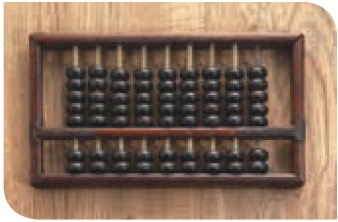
\includegraphics[width=.5\linewidth]{./Images/abaco.jpg}
    \caption{Initial condition}
    \vspace{4ex}
  \end{minipage}%%
  \begin{minipage}[b]{0.5\linewidth}
    \centering
    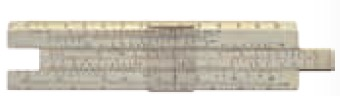
\includegraphics[width=.5\linewidth]{./Images/regla_calculo.jpg}
    \caption{Rupture}
    \vspace{4ex}
  \end{minipage}
  \begin{minipage}[b]{0.5\linewidth}
    \centering
    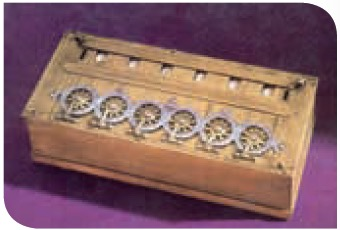
\includegraphics[width=.5\linewidth]{./Images/pascalina.jpg}
    \caption{DFT, Initial condition}
    \vspace{4ex}
  \end{minipage}%% 
  \begin{minipage}[b]{0.5\linewidth}
    \centering
    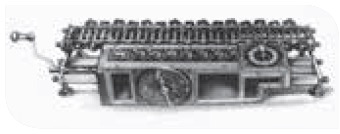
\includegraphics[width=.5\linewidth]{./Images/maquina_Leibniz.jpg}
    \caption{DFT, rupture}
    \vspace{4ex}
  \end{minipage}
\end{figure}
% \centering
% \includegraphics[width=0.5\textwidth]{}
% \includegraphics[width=0.5\textwidth]{}
% \includegraphics[width=0.5\textwidth]{}
% \includegraphics[width=0.5\textwidth]{}
% \caption{a) \'abaco, b) Regla de c\'alculo , c) Pascalina, d) M\'aquina de Leibniz. Evoluci\'on de instrumentos para el c\'alculo.}

En el siglo XVII se inventaron las primeras calculadoras mec\'anicas, las cuales
funcionaban a base de engranes y palancas.
En 1639 el matem\'atico, f\'isico y fil\'osofo \textbf{Blaise Pascal (1623-1662)}
cre\'o la ``Pascalina'', instrumento para sumar y
restar que constaba de una serie de engranajes marcados con los n\'umeros del 0
al 9; cuando un engrane daba una vuelta completa,
en el siguiente engrane se sumaba una unidad.
Treinta años despu\'es el matem\'atico \textbf{Gottfried Wilhelm Leibniz
  (1646-1716)} construy\'o una calculadora similar a la
Pascalina que adem\'as de sumar y restar, multiplicaba y divid\'ia; tambi\'en usaba
engranes, los n\'umeros para los c\'alculos se
introduc\'ian por medio de botones y con una manivela se hac\'ia girar todo el
mecanismo (figura 1.2).
Con el paso de los años este tipo de calculadoras se fueron perfeccionando, y
ya en el siglo su uso era com\'un en las tiendas
de autoservicio, incluso se fabricaron calculadoras mec\'anicas compactas que
cab\'ian en la palma de la mano, pero eran muy
costosas. En la d\'ecada de los cincuenta apareci\'o la primera calculadora de
transistores, que era del tamaño de un escritorio.
A finales de los cincuenta surgieron las primeras calculadoras b\'asicas
totalmente electr\'onicas con precios elevad\'isimos,
cerca de \$80,000 d\'olares. Fue hasta inicios de los años setenta que varias
compañ\'ias produjeron calculadoras que funcionaban
con pilas y a precios accesibles, las cuales se vendieron por todo el mundo. En
1973 aparecieron las calculadoras cient\'ificas,
que no s\'olo hac\'ian operaciones b\'asicas, sino que calculaban ra\'ices y potencias
de distintos valores, y utilizaban funciones
trigonom\'etricas y otras m\'as complejas las cuales estudiar\'as en tus cursos m\'as
avanzados de matem\'aticas. A finales del siglo XX
se incorporaron las celdas solares, por lo que ahora contamos con calculadoras
que no necesitan bater\'ias. Actualmente las
calculadoras son capaces de resolver operaciones superiores, ecuaciones y hasta
trazar gr\'aficas.
?`C\'omo se mide el tiempo?

El tiempo es una cantidad f\'isica que nos permite enmarcar el cambio y ordenar
los sucesos en secuencias, estableciendo un pasado,
un presente y un futuro.

Figura 1.4. Actualmente el segundo se define a partir de fen\'omenos a nivel
at\'omico.

La unidad de tiempo ``año''” tiene su origen en el periodo que la Tierra tarda
en dar una vuelta alrededor del Sol; un ``d\'ia''”
se refiere al tiempo en que la Tierra completa una vuelta sobre su propio eje,
y que antiguamente se determinaba como el tiempo
que transcurr\'ia entre una y otra salida del Sol. Ya desde la Antigüedad los
egipcios y sumerios dividieron el d\'ia en 24 horas,
12 para la luz diurna y 12 para la noche; la divisi\'on entre minutos y segundos
(figura 1.4) surgi\'o a partir de la necesidad
de medir los fen\'omenos celestes con m\'as precisi\'on, y fue en la Edad Media
cuando estas \'ultimas unidades se aplicaron para la
medici\'on del tiempo. Por cierto, la palabra \textbf{minuto}, tiene su origen en
la palabra latina \emph{minutus}, que significa ``peque\~no''”,
y \textbf{segundo} se deriva de secundus, que significa ``el que va despu\'es del
primero'', por lo que un segundo  es lo que
sigue en pequeñez a un minuto. Los subm\'ultiplos del segundo, como el
milisegundo y el microsegundo, se emplean para mediciones
muy precisas, como en fen\'omenos a nivel at\'omico.

La unidad oficial para medir el tiempo en el Sistema Internacional de Unidades
(SI) es el segundo (s\'imbolo: s), pero
cotidianamente utilizamos otras unidades, como minutos, horas, d\'ias, años,
entre otros. Observa las equivalencias.
\begin{multicols}{3}
  60 segundos = 1 minuto
  365.256 d\'ias = 1 año
  100 años = 1 siglo
  60 minutos = 1 hora
  5 años = 1 lustro
  1 000 años = 1 milenio
  24 horas = 1 d\'ia
  10 años = 1 d\'ecada
\end{multicols}
Tambi\'en hay subm\'ultiplos del segundo que se basan en el sistema decimal:

1 segundo = 10 decisegundos = 100 centisegundos = 1000 milisegundos

% \begin{questions}
%   \question[10] ?`Cu\'antos meses y d\'ias has vivido desde que naciste hasta hoy?
%   \question[10] ?`Cu\'antas horas hay en un siglo?
%   \question[10] ?`Cu\'antos milisegundos tiene un minuto?

%   \question[10] Elige la respuesta correcta.

%   \renewcommand{\labelenumi}{\Alph{enumii}}
%   \begin{enumerate}
%     \item Los seres humanos se distinguen de los animales por su capacidad de
%           cambiar su entorno creando herramientas que le facilitan tareas o mejoran su
%           condici\'on de vida, a esto le llamamos\dots

%           \begin{choices}
%             \choice F\'isica
%             \choice Cultura
%             \choice Meditaci\'on
%           \end{choices}
%     \item La herramienta m\'as antigua que conocemos, creada para facilitar los
%           c\'alculos matem\'aticos es \dots

%           \begin{choices}
%             \choice el \'abaco
%             \choice El comp\'as
%             \choice La calculadora
%             \choice La regla de c\'alculo
%           \end{choices}
%     \item Las primeras calculadoras como la inventada por Blaise Pascal en 1639
%           funcionaban a base de \dots

%           \begin{choices}
%             \choice circuitos
%             \choice engranajes
%             \choice cuentas deslizables
%             \choice regletas deslizables
%           \end{choices}
%     \item  En 1973 apareci\'o este instrumento capaz de realizar c\'alculos
%           complejos como ra\'ices, potencias y  funciones trigonom\'etricas.

%           \begin{choices}
%             \choice \'abaco
%             \choice Calculadora b\'asica
%             \choice Calculadora cient\'ifica
%             \choice Regletas de c\'alculo avanzado
%           \end{choices}
%   \end{enumerate}

%   \question[10] Relaciona los siguientes elementos.

%   \begin{minipage}{0.5\linewidth}
%     \begin{enumerate}
%       \item Inventor de la regla de c\'alculo.
%       \item Inventor de una calculadora similar a la pascalina que pod\'ia
%             multiplicar y dividir.
%       \item Este tipo de calculadora apareci\'o en los años cincuenta y fue
%             totalmente electr\'onica con precios cerca de \$80 000 d\'olares.
%       \item Este tipo de calculadora resuelve operaciones con ra\'ices y
%             potencias de distintos valores. Apareci\'o en 1973.
%       \item Calculadora del tamaño de un escritorio.
%     \end{enumerate}
%   \end{minipage}
%   \begin{minipage}{0.4\linewidth}

%     \begin{choices}
%       \choice Calculadora b\'asica \vspace{0.5cm}
%       \choice Gottfried Wilhelm Leibnitz  \vspace{0.5cm}
%       \choice William Oughtred	  \vspace{0.5cm}
%       \choice Calculadora de transistores    \vspace{0.5cm}
%       \choice Calculadora cient\'ifica   \vspace{0.5cm}
%     \end{choices}

%   \end{minipage}

%   \question[10] Ordena los nombres de los creadores de instrumentos de c\'alculo,
%   del m\'as antiguo al m\'as reciente.

%   \begin{enumerate}
%     \item Gottfried Leibniz
%     \item William Oughtred
%     \item Blaise Pascal
%   \end{enumerate}
% \end{questions}
\section{Velocidad y aceleraci\'on}
\subsection{El movimiento de los objetos}
\subsection{La velocidad y la rapidez}
\subsection{Gr\'aficas que representan la velocidad (desplazamiento vs. tiempo)}
\subsection{La aceleraci\'on como cambio de la velocidad}

\section{Movimiento ondulatorio}
\subsection{Ondas para ver}

\section{Concepto de fuerza}
\subsection{La fuerza como interacci\'on entre los objetos}
\subsection{Suma de fuerzas}
\subsection{M\'aquinas simples}

\section{Leyes de Newton}
\subsection{Primera Ley de Newton}
\subsection{Segunda Ley de Newton}
\subsection{Tercera Ley de Newton}

\section{La aportaci\'on de Newton}
\subsection{Ley de Gravitaci\'on Universal}
\subsection{Newton, vida y obra, sus aportaciones para la ciencia}
\subsection{El movimiento regular de los cuerpos del Sistema Solar: las leyes de Kepler}

\chapter{}

\section{La energ\'ia y sus manifestaciones}
\subsection{Tipos de energ\'ia}

\begin{center}
  % \boxabstract{
  %   Analiza la energ\'ia mec\'anica (cin\'etica y potencial) y describe casos donde
  %   se conserva.
  % }
\end{center}

Analiza el texto y responde.
?`Conoces la teor\'ia del meteorito que caus\'o la extinci\'on de los dinosaurios
hace 65 millones de años? Los cient\'ificos dicen que cay\'o sobre la pen\'insula
de Yucat\'an y que la energ\'ia del impacto era equivalente a la que liberar\'ian
5,000 millones de bombas at\'omicas como la lanzada sobre Nagasaki. El
meteorito debi\'o tener un di\'ametro mayor a 10 km y moverse a 54,000 km/h.
Debido al impacto se form\'o un cr\'ater de 100 km de di\'ametro, se elev\'o
la temperatura en esa zona y se produjo un enorme resplandor: fragmentos
incandescentes, tanto del meteorito como del terreno donde cay\'o, salieron
disparados provocando incendios en distintas partes del planeta.
Como consecuencia del choque se levant\'o una gran cantidad de polvo
que cubri\'o el cielo e impidi\'o el paso de la luz solar, lo que limit\'o la
fotos\'intesis de las plantas y alter\'o las redes tr\'oficas.
\begin{itemize}
  \item La luz y el calor son manifestaciones de la energ\'ia. ?`Qu\'e piensan que
        provoc\'o la formaci\'on de
        fragmentos incandescentes al caer el meteorito? ?`De
        d\'onde proven\'ia la energ\'ia que caus\'o la luz y el fuego durante el impacto?
  \item Si el meteorito hubiera sido m\'as pequeño, ?`habr\'ia producido tanta
        destrucci\'on? ?`Y si se
        hubiera movido con una rapidez menor?
  \item ?`En qu\'e situaciones de la vida cotidiana han escuchado la palabra
        \emph{energ\'ia}? ?`En esas
        situaciones hay algo que cambie o se transforme? ?`Podr\'ian decir qu\'e es la
        energ\'ia?
\end{itemize}

% \begin{questions}
%   \question Es probable que t\'u, tu familia y tus amigos utilicen la palabra ``energ\'ia'' de
%   manera cotidiana: saben que si la energ\'ia el\'ectrica ``se va'',
%   la televisi\'on, el refrigerador o la licuadora no funcionan. Es posible
%   que hayan escuchado que en las noticias se refieren a los combustibles f\'osiles
%   como energ\'eticos, y que entre ellos est\'a el petr\'oleo
%   y el gas natural, o que en alg\'un comercial hablen de pilas que ``dan m\'as
%   energ\'ia''. Seguramente sabes que si la bater\'ia de un tel\'efono
%   m\'ovil se agota, hay que conectarlos a una toma de corriente el\'ectrica. En tu
%   curso de Ciencias y tecnolog\'ia 1 aprendiste que incluso
%   nosotros necesitamos energ\'ia para realizar nuestras funciones vitales, la cual
%   obtenemos de los alimentos mediante la digesti\'on.

%   Pero, ?`qu\'e es la energ\'ia?, ?`c\'omo se manifiesta? ?`C\'omo se relacionan la energ\'ia
%   y el
%   movimiento, por ejemplo, para que se mueva un autom\'ovil? La energ\'ia tiene
%   manifestaciones muy diversas y es casi seguro que hayas experimentado muchas de
%   ellas.
%   \question Relaciona los tipos de energ\'ia con sus fuentes. En tu cuaderno
%   anota al menos
%   un ejemplo en el que se utilice o aplique cada tipo de energ\'ia.
%   \begin{figure}[H]
%     \centering
%     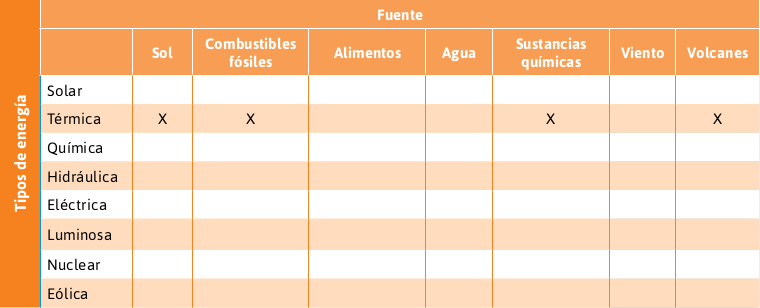
\includegraphics[width=0.8\textwidth]{./Images/tablaS7_tipos_fuentes.png}
%   \end{figure}
%   A partir de tus ejemplos, examina qu\'e usos se dan a la energ\'ia. ?`Qu\'e tienen
%   en
%   com\'un?, ?`en ellos se transforma o modifica algo? Analiza con tus compañeros
%   las respuestas y lo que entienden por energ\'ia; en un texto expresen el
%   significado del t\'ermino.
% \end{questions}

\subsubsection{?`Qu\'e es la energ\'ia?}
?`Si la energ\'ia nos parece un concepto tan familiar por qu\'e resulta tan
dif\'icil definirlo? Tal vez porque la energ\'ia es un concepto abstracto: no
es un objeto o una sustancia. A diferencia de la materia, no podemos
ver ni tocar la energ\'ia y, sin embargo, es uno de los conceptos fundamentales
de la ciencia, y quiz\'a el m\'as importante de toda la f\'isica (figura 2.2). Te
sorprender\'a saber que incluso a Isaac Newton se le escap\'o
el concepto de energ\'ia, y que m\'as de un siglo despu\'es de su muerte los
cient\'ificos a\'un cuestionaban su existencia.
Sin embargo, lo que todas las formas de energ\'ia tienen en com\'un es
que pueden transformarse de una forma a otra; por ejemplo, la energ\'ia
el\'ectrica puede provocar movimiento y transformarse en calor que quiz\'a
has percibido al encender una licuadora o un ventilador: las aspas se mueven y
despu\'es de un tiempo el aparato se calienta. Estas transformaciones
pueden cuantificarse, y el n\'umero que resulta es siempre el mismo sin importar
la cantidad de transformaciones que sucedan.
Por ahora definiremos la energ\'ia como la capacidad que tiene una
persona, un objeto, una m\'aquina, un robot, un animal, etc\'etera, para
interactuar con otros objetos. Siempre que hablamos de energ\'ia la relacionamos
con alg\'un cambio, presente o futuro, en los objetos a los que nos
referimos: cambian de estado de movimiento, de forma, de composici\'on (por
ejemplo, durante la combusti\'on), de lugar, etc\'etera.

\subsubsection{La energ\'ia mec\'anica}
?`C\'omo se modifica el estado de reposo o de movimiento de un objeto? En efecto,
con la aplicaci\'on de una fuerza; por tanto, y de acuerdo con la definici\'on
de energ\'ia, existe una estrecha relaci\'on entre la energ\'ia y la fuerza. En todo
cambio de posici\'on o de movimiento de un objeto la energ\'ia est\'a involucrada,
pero para que se d\'e dicho cambio debe tener lugar un desplazamiento.
Si un coche se mueve con cierta rapidez y acelera hasta alcanzar una
rapidez mayor, requerir\'a energ\'ia (la cual proporciona el combustible); el
veh\'iculo, por tanto, est\'a cambiando su estado de movimiento y se realiza
un desplazamiento.
Si una caja inicialmente se encuentra en el piso, cuando se coloca en lo
alto de un librero tiene un cambio en su posici\'on: para subirla se requiri\'o
una cierta energ\'ia y hubo un desplazamiento.
De esta manera, el cambio en el movimiento o en la posici\'on de un objeto
se comprende no s\'olo a partir del concepto de fuerza, sino tambi\'en con base
en el de energ\'ia. La energ\'ia relacionada con el movimiento o la posici\'on de
un objeto se conoce como energ\'ia mec\'anica, y se manifiesta cuando cambia
su estado de movimiento o su posici\'on al aplicarle una determinada fuerza.
Para cuantificar la energ\'ia mec\'anica definiremos dos conceptos nuevos:
energ\'ia cin\'etica y energ\'ia potencial.

\subsubsection{Energ\'ia cin\'etica}
Si has andado en bicicleta, jugado futbol o competido en una carrera, sabr\'as
que despu\'es del ejercicio te sientes cansado. ?`Sab\'ias que Michel Phelps
(1985), nadador estadounidense que ha ganado 28 medallas ol\'impicas, para
entrenar com\'ia lo mismo que cinco adultos? Es un hecho que para llevar a
cabo un esfuerzo f\'isico se requiere energ\'ia, y por eso, despu\'es de
ejercitarnos, sentimos hambre. Con lo anterior queremos decir que el movimiento
est\'a relacionado con la energ\'ia. La energ\'ia que posee un cuerpo debido a
su movimiento se conoce como energ\'ia cin\'etica (del griego kinetos: que se
mueve). Si te has golpeado con un bal\'on de futbol o te has golpeado un dedo
del pie contra un mueble mientras caminas, entonces has sentido los efectos de
la energ\'ia cin\'etica.

Como experimentaste, la energ\'ia cin\'etica de un cuerpo en movimiento depende de
dos variables o magnitudes f\'isicas: su masa (m) y su rapidez (v). La ecuaci\'on
que relaciona ambas variables y define a la energ\'ia cin\'etica ($E_C$) es:

\begin{equation*}
  E_c=\frac{1}{2}mv^2
\end{equation*}

% Las unidades de la energ\'ia cin\'etica, derivadas a partir de su ecuaci\'on, son las
% de masa por las de rapidez al cuadrado: kg m^2/s^2, que corresponden a las
% unidades de la energ\'ia en el SI;es decir, al joule (J). Como sabes, la unidad de fuerza es el
% newton (N), y 1 N equivale a 1 kg m/s$^2$, de manera que:

\( 1 J = 1 kg m^2/s^2 = 1 Nm \)

% \begin{questions}
%   \question Considera un carro de la montaña rusa de 300 kg en el que suben
%   ocho
%   personas con una masa promedio de 60 kg. Si en la parte m\'as baja de
%   una curva descendente el carro lleva una rapidez de 120 km/h:
%   \begin{oneparchoices}
%     \choices ?`Cu\'al es su energ\'ia cin\'etica en ese instante?
%     \choices ?`En qu\'e lugares o situaciones la energ\'ia cin\'etica ser\'a cero?
%     \choices ?`C\'omo cambiar\'ia la energ\'ia cin\'etica del carro en la parte m\'as baja
%     de una curva descendente si se suben menos personas?
%   \end{oneparchoices}
%   \question ?`Cu\'al es la masa de un avi\'on que se desplaza a 800 km/h si su
%   energ\'ia cin\'etica es de 30,000,000 J?
%   \question ?`Qui\'en utiliza m\'as energ\'ia, una persona que sube a un edificio de
%   cinco pisos o una que escala a la cima del volc\'an Popocat\'epetl? ?`Por qu\'e?
%   \question ?`Cu\'al tiene mayor energ\'ia, una piedra en reposo en el piso o una
%   con la misma masa que se encuentra a una altura de 5 m tambi\'en en reposo? ?`Por
%   qu\'e?
%   \question ?`Qu\'e objeto producir\'ia mayores cambios al interactuar con otros
%   debido a la atracci\'on gravitacional, uno de menor o uno de mayor masa?
%   \question ?`Un cuerpo puede tener energ\'ia aun sin moverse? Explica.
% \end{questions}

\subsubsection{Energ\'ia potencial}
Si colocas un libro en la parte superior de un librero, utilizas una fuerza y
lo desplazas cierta distancia; por tanto, requieres cierta energ\'ia para llevar
a cabo el cambio en su posici\'on, pero el libro, aun inm\'ovil, interact\'ua con la
Tierra (lo que se
manifiesta por su peso), puede caer y desplazarse una distancia. Debido a esta
posibilidad se dice que el libro tiene energ\'ia potencial. As\'i, podemos definir
la energ\'ia
potencial gravitacional como la energ\'ia que tiene un cuerpo en virtud de su
posici\'on
y que est\'a relacionada con la fuerza de gravedad.

La energ\'ia potencial depende de la altura del objeto con respecto a un marco de
referencia, que puede ser la superficie terrestre, la mesa de trabajo, el
pupitre,
de modo que todo objeto que se encuentre en el origen de nuestro marco de
referencia tendr\'a energ\'ia potencial gravitacional igual a cero. Mientras m\'as
alta sea la posici\'on de un objeto en relaci\'on con el origen, mayores ser\'an los
cambios que pueda
producir al interactuar con otros objetos y, por tanto, mayor ser\'a su energ\'ia
potencial
gravitacional.
La energ\'ia potencial tambi\'en depende de la masa de un cuerpo. As\'i, la
ecuaci\'on para el c\'alculo de la energ\'ia potencial gravitacional ($E_P$) involucra
a la masa de un cuerpo (m), la altura a la que se encuentra con respecto al
marco de referencia (h) y la aceleraci\'on de la gravedad (g):
\begin{equation*}
  E_p=mgh
\end{equation*}
La unidad de la energ\'ia potencial, como la de la energ\'ia cin\'etica, es el de un
objeto se relaciona con
su posici\'on.
joule (J). ?`Puedes demostrarlo a partir de la ecuaci\'on?
Antes dijimos que la energ\'ia mec\'anica ($E_m$) de un cuerpo est\'a en funci\'on de su
movimiento y su posici\'on, es decir, la energ\'ia mec\'anica depende de la energ\'ia
cin\'etica y de la energ\'ia potencial de acuerdo con la siguiente expresi\'on:
\begin{equation*}
  E_m=E_c+E_p
\end{equation*}

\subsubsection{Ejercicios}
% \begin{questions}
%   \question ?`Cu\'al es la masa de un objeto que est\'a a una altura de 100 m y cuya
%   energ\'ia potencial es de 1 000 J?
%   \question ?`Puede un objeto en una playa tener la misma energ\'ia potencial
%   gravitacional que otro de la misma masa que est\'a en la Ciudad de M\'exico a una
%   altitud de 2 240 m sobre el nivel del mar? Explica.
%   \question ?`C\'omo es la energ\'ia potencial de un avi\'on de carga que viaja a una
%   altura de 4 000 m a 900 km/h y que tiene una masa de 500 toneladas con respecto
%   a un jet de 250 toneladas que viaja con una rapidez de 1 800 km/h a la misma
%   altura?
%   \question Calcula la cantidad de energ\'ia mec\'anica total de un autom\'ovil que
%   sube una montaña, el cual tiene una masa de una tonelada, se localiza a una
%   altura de 500 m y lleva una rapidez de 50 km/h.


%   Retoma el problema de la situaci\'on de la secci\'on Inicio y verifica si tus
%   respuestas fueron correctas. Despu\'es responde.
%   \begin{choices}
%     \choice ?`Es posible que un meteorito como el que cay\'o en la pen\'insula de
%     Yucat\'an hace 60 millones de años haya provocado una cat\'astrofe mundial? ?`Por
%     qu\'e?
%     \choice ?`Qu\'e tipo de energ\'ia ten\'ia el meteorito? Explica.
%     \choice ?`Esa energ\'ia pudo causar la gran cantidad de calor y luz que se supone
%     se gener\'o durante el impacto? ?`Por qu\'e?
%     \choice ?`Qu\'e entiendes por energ\'ia?
%   \end{choices}
% \end{questions}
\subsection{La conservaci\'on de la energ\'ia mec\'anica}

Una actividad muy popular entre algunos j\'ovenes es el skate, donde el skater
se desliza sobre una patineta. Aunque el skate puede practicarse en cualquier
lugar, existen complejos especiales, conocidos como skateparks, equipados
con rampas de varios tipos. El half pipe (medio tubo) es una rampa en forma
de ``U'' especialmente diseñada para ``surfear en seco''.
El skater se desliza desde el borde del half pipe y, haciendo gala de habilidad y equilibro, intenta alguna rutina de trucos que asombren a su p\'ublico:
el skate es un deporte de exhibici\'on, pero, desde otra perspectiva, en \'el hay
mucha f\'isica involucrada.
%\begin{oneparchoices}
%  \choice Si el skater se desliza desde el borde del half pipe, sin impulsarse, alcanza el lado opuesto y vuelve, iniciando un movimiento oscilatorio. ?`En qu\'e puntos su energ\'ia potencial alcanza sus valores m\'aximos y m\'inimos?
%  \choice Y qu\'e hay de la energ\'ia cin\'etica, ?`en qu\'e puntos alcanza sus valores m\'aximos  y m\'inimos? ?`En qu\'e puntos se logra la mayor rapidez y en cu\'ales la m\'inima?
%  \choice Si cuando se lanza el skater s\'olo posee energ\'ia potencial, ?`de d\'onde ``sale'' su energ\'ia cin\'etica?
%\end{oneparchoices}

\subsubsection{La energ\'ia se transforma}
Hemos hablado mucho acerca de la energ\'ia, pero ?`ya te diste cuenta de que
todav\'ia
no se ha dado una definici\'on precisa y definitiva de lo que es? Ya sabes
bastante sobre
la energ\'ia: que se manifiesta de diversas formas, que existen muchas fuentes y
varios
tipos de energ\'ia e incluso que hay f\'ormulas matem\'aticas para calcularla.
Entonces,
?`qu\'e es la energ\'ia?, ?`cu\'al es su definici\'on? Te asombrar\'a saberlo: actualmente
los f\'isicos contin\'uan sin saber qu\'e es la energ\'ia, y quiz\'a ya no est\'en
interesados en plantear
una definici\'on definitiva. En realidad no importa. Lo que verdaderamente
interesa
saber acerca de la energ\'ia es c\'omo se comporta, c\'omo se transforma.
Veamos c\'omo se comporta, en concreto, la energ\'ia mec\'anica.

%\begin{mybox}{0.60\linewidth}{
%\begin{comfortaa}
%    \color{white} Pr\'actica
%\end{comfortaa}
%  }
%  \begin{questions}
%    \question El edificio m\'as alto del mundo -hasta el momento- es
%    el Burj Khalifa, ubicado a orillas del golfo P\'ersico en Dubai,
%    ciudad de Emiratos \'arabes Unidos: mide 828 m de altura.
%    Imagina que desde una altura igual a la de la torre se
%    deja caer una pelota de 100 g y considera que no hay
%    fricci\'on del aire ni variaciones en el valor de la aceleraci\'on
%    de la gravedad.
%    \begin{oneparchoices}
%      \choices ?`Cu\'anto tiempo tardar\'a la pelota en llegar al suelo?
%      \choices ?`Qu\'e velocidad tendr\'a justo antes de tocarlo?
%      \choices Calculen en equipo los resultados. Estos problemas no son nuevos
%      para ustedes, pero vamos un poco m\'as all\'a: observar lo que ocurre con la
%      energ\'ia de la pelota.
%      \choices Calculen la energ\'ia cin\'etica, potencial y mec\'anica de la pelota
%      cada segundo, desde que se suelta, es decir, desde t = 0 s, y para el valor del
%      tiempo de ca\'ida. Anoten los resultados en una tabla como la siguiente y
%      graf\'iquenlos.
%      \choices Aqu\'i presentamos como ejemplo la gr\'afica correspondiente a t = 5 s.
%      Observen que incluimos una gr\'afica circular (figura a) y una de barras (figura
%      b) para optimizar el an\'alisis.
%      \choices ?`Cu\'al es el valor de la energ\'ia potencial de la pelota E al
%      momento de soltarla, es decir, en t = 0 s? ?`Cu\'anto vale la energ\'ia cin\'etica?,
%      ?`y la energ\'ia mec\'anica total?
%      \choices ?`Qu\'e valor tiene la energ\'ia potencial de la pelota un instante
%      antes de que toque el piso? ?`Cu\'anto vale la energ\'ia cin\'etica?, ?`y la energ\'ia
%      mec\'anica total?
%      \choices Ordenen las gr\'aficas seg\'un la secuencia temporal y obs\'ervenlas.
%      ?`Qu\'e notan?, ?`c\'omo cambia la energ\'ia potencial en el transcurso del tiempo?,
%      ?`la cin\'etica?, ?`y la total?
%      \choices ?`Qu\'e pasa con la energ\'ia cin\'etica cuando cambia la potencial? ?`Qu\'e
%      relaci\'on hay entre estas cantidades?
%      \choices ?`Cu\'ales son sus conclusiones? Reg\'istrenlas en su cuaderno.
%    \end{oneparchoices}
%  \end{questions}
%\end{mybox}
Ya conocemos cuatro leyes de la F\'isica. No todas las leyes f\'isicas
se resumen en f\'ormulas matem\'aticas. Ahora consideraremos una ley
relacionada con la energ\'ia; quiz\'a -si te pones un poco curioso- te
asombre su formulaci\'on porque es un poco distinta de las anteriores.
Richard Feynman (1918-1988), uno de los m\'as ingeniosos, destacados
y extravagantes f\'isicos de la historia y ganador del premio Nobel de
F\'isica en 1965, la explicaba as\'i:
Existe una cierta cantidad, que llamamos energ\'ia, que no cambia
cuando en la naturaleza ocurre un cambio. Es una idea de lo m\'as abstracta
porque es un principio matem\'atico que dice que hay una cantidad que no cambia
cuando algo sucede. No es la descripci\'on de un
mecanismo ni algo concreto. Es tan s\'olo un hecho extraño el que seamos capaces
de calcular un n\'umero, y que al volver a calcularlo despu\'es de observar las
piruetas de la naturaleza, \'este sea el mismo.
\section{Los modelos en la ciencia}
\subsection{Explicaci\'on de los fen\'omenos de la naturaleza a partir de modelos}
\subsection{Ideas en la historia entorno a la estructura de la materia}
\subsection{Aspectos b\'asicos del modelo cin\'etico de part\'iculas}

\section{Cambios de estado de la materia y el modelo cin\'etico}
\subsection{Propiedades de la materia: forma, volumen, estados de agregaci\'on, compresibilidad, etc\'etera}
\subsection{Cambios de estado de agregaci\'on}

\section{Temperatura y equilibrio t\'ermico}
\subsection{Temperatura}
\subsection{Calor y temperatura}

\section{Calor como energ\'ia}
\subsection{Energ\'ia t\'ermica}
\subsection{Calor y otras formas de energ\'ia}
\subsection{Energ\'ia el\'ectrica y medio ambiente}

\section{Interacciones el\'ectricas}
\subsection{Fen\'omenos electrost\'aticos}

\section{El modelo at\'omico de la materia}
\subsection{Descripci\'on macrosc\'opica y microsc\'opica del Universo}
\subsection{Desarrollo hist\'orico del modelo at\'omico}
\subsection{Caracter\'isticas del \'atomo}

\chapter{}

\section{Corriente el\'ectrica y magnetismo}
\subsection{Corriente el\'ectrica y magnetismo}
\subsection{Electromagnetismo}

\section{Electricidad y magnetismo: ondas electromagn\'eticas}
\subsection{Relaci\'on entre electricidad y magnetismo}
\subsection{Inducci\'on electromagn\'etica}
\subsection{Generaci\'on de ondas electromagn\'eticas}
\subsection{La luz visible}

\section{Electricidad y temperatura en sistemas biol\'ogicos}
\subsection{La f\'isica del cuerpo humano}

\section{Ciencia, tecnolog\'ia y sociedad}
\subsection{Ciencia y tecnolog\'ia aplicada a la salud}
\subsection{Ciencia y tecnolog\'ia en el mundo actual}

\section{F\'isica y conocimiento del Universo}
\subsection{La estructura del Universo}
\subsection{?`C\'omo se estudia el Universo?}
\subsection{Los mecanismos de las estrellas}

\section{El Sistema Solar}
\subsection{Caracter\'isticas y exploraci\'on del Sistema Solar}
\subsection{Origen del Sistema Solar}

\section{Origen y evoluci\'on del Universo}
\subsection{Teor\'ia de la Gran Explosi\'on}

\end{document}